\chapter{Linear Multistep Methods}
\label{chap:lmm}

\section{Introduction and Motivation}
\label{sec:lmm:intro}
Many initial-value problems
\begin{equation}
  y'(t)=f\left(t,y(t)\right), \qquad y(t_0)=y_0,
  \label{eq:ivp}
\end{equation}
must be solved repeatedly in science and engineering.
One-step methods (Euler, Runge-Kutta) march forward using \emph{only the most recent point}.
\emph{Linear multistep methods (LMMs)} reuse computed information from several previous time levels.
Think of them as driving a car while glancing not only at the speedometer right now, but also remembering the readings from the last few seconds: with more historical data you can estimate the distance travelled more accurately without pressing the gas pedal again (\autoref{fig:lmm-history}).

\begin{figure}[htbp]
  \centering
  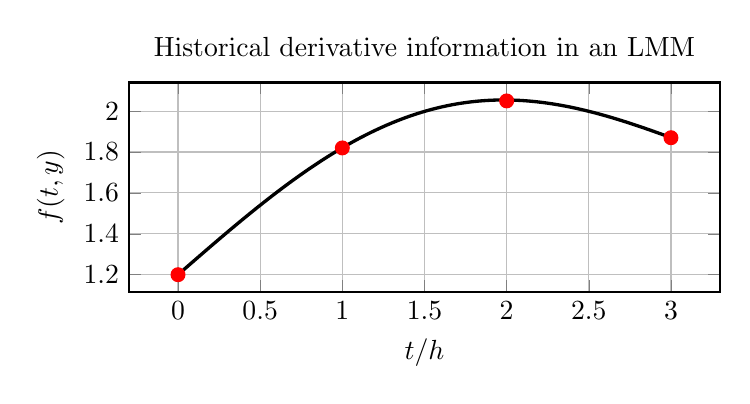
\begin{tikzpicture}
    \begin{axis}[
        width=0.75\textwidth,
        height=0.35\textwidth,
        xlabel={$t/h$}, ylabel={$f(t,y)$},
        title={Historical derivative information in an LMM},
        grid=both,
        domain=0:3,
        samples=100,
        axis line style={thick}]
      \addplot[very thick] {0.5*sin(deg(x))+1.2+0.2*x};
      \addplot[only marks, mark=*, mark size=2.5pt, red] coordinates
        {(0,1.2) (1,1.82) (2,2.05) (3,1.87)};
    \end{axis}
  \end{tikzpicture}
  \caption{An LMM predicts the future integral of $f$ using derivative values stored from several past steps.}
  \label{fig:lmm-history}
\end{figure}

Compared with high-order Runge-Kutta methods, multistep schemes:
\begin{itemize}
  \item offer the \textbf{same maximal algebraic order} for fewer expensive evaluations of~$f$;
  \item separate \emph{accuracy} (the number of steps~$k$) from the \emph{cost per step} (still one right-hand side evaluation for explicit methods);
  \item trade accuracy for \emph{reduced stability}, making the analysis of root locations in the complex plane a central theme.
\end{itemize}

\section{General Formulation of a k-Step Linear Multistep Method}
\label{sec:lmm:general}

\begin{definition}{Linear Multistep Method}{lmm}
  Let $\{t_n\}_{n\ge0}$ be an equidistant grid with fixed step $h=t_{n+1}-t_n>0$.
  A \emph{$k$-step linear multistep method (LMM)} approximates the solution of \eqref{eq:ivp} through the recurrence
  \begin{equation}
    \sum_{j=0}^{k}\alpha_j\,y_{n+j} = h\sum_{j=0}^{k}\beta_j\,f_{n+j}, \qquad\text{where }f_{n+j}=f(t_{n+j},y_{n+j}),
    \label{eq:lmm}
  \end{equation}
  with constant real coefficients $\alpha_j,\beta_j$ satisfying $\alpha_k\neq0$ and $\gcd\bigl(\{\alpha_j\}_{0}^{k}\bigr)=1$.
  We call the method \emph{explicit} if $\beta_k=0$ and \emph{implicit} otherwise.
\end{definition}

\subsection{Characteristic Polynomials and Root Condition}
\label{sec:lmm:root}
Define the polynomials
\[
  \rho(\zeta)=\sum_{j=0}^{k}\alpha_j\,\zeta^j,
  \qquad
  \sigma(\zeta)=\sum_{j=0}^{k}\beta_j\,\zeta^j.
\]
The \textbf{root condition} states that all roots of $\rho$ lie in $|\zeta|\le1$; any root on the unit circle must be \emph{simple} (i.e., has multiplicity one $j = 1$).
This condition is essential for zero-stability and therefore convergence (\autoref{sec:lmm:convergence}).

\section{Error Analysis}

\subsection{Local Truncation Error, Order and Consistency}
\label{sec:lmm:lte}

\begin{definition}{Local Truncation Error (LTE)}{lmm:lte}
  Suppose the exact solution $y(t)$ of \eqref{eq:ivp} is inserted into \eqref{eq:lmm}.
  The resulting defect
  \[
    \tau_{n+k} := \displaystyle \sum_{j=0}^{k}\alpha_j\,y(t_{n+j})-h\sum_{j=0}^{k}\beta_j\,y'(t_{n+j})
  \]
  is called the \emph{local truncation error}.
  The method is of (algebraic) \emph{order~$p$} if $\tau_{n+k}= \mathcal{O}(h^{p+1})$ as $h\to0$.
\end{definition}

\begin{definition}{Consistency}{lmm:consistency}
  A linear multistep method is \emph{consistent} if its local truncation error $\tau_{n+k} \to 0$ as $h \to 0$ for all sufficiently smooth $y(t)$.
  Equivalently, the method is consistent if
  \[
    \sum_{j=0}^{k} \alpha_j = 0
    \qquad \text{and} \qquad
    \sum_{j=0}^{k} j\,\alpha_j = \sum_{j=0}^{k} \beta_j.
  \]
\end{definition}

\begin{example}{Exam H2022: Problem 5 d)}{}
  Consider the method
  \[
    3y_{n+2} - 4y_{n+1} + y_n = 2h f_{n+2}.
  \]
  This is a two-step ($k=2$) linear multistep method with coefficients:
  \[
    \alpha_0 = 1,\quad \alpha_1 = -4,\quad \alpha_2 = 3;\qquad
    \beta_0 = 0,\quad \beta_1 = 0,\quad \beta_2 = 2.
  \]

  \textbf{Consistency:}
  A linear multistep method is consistent if
  \[
    \sum_{j=0}^k \alpha_j = 0
    \qquad \text{and} \qquad
    \sum_{j=0}^k j\,\alpha_j = \sum_{j=0}^k \beta_j.
  \]
  Compute:
  \begin{align*}
    \sum_{j=0}^2 \alpha_j    & = 1 + (-4) + 3 = 0,                            \\
    \sum_{j=0}^2 j\,\alpha_j & = 0\cdot1 + 1\cdot(-4) + 2\cdot3 = -4 + 6 = 2, \\
    \sum_{j=0}^2 \beta_j     & = 0 + 0 + 2 = 2.
  \end{align*}
  Both conditions are satisfied, so the method is \textbf{consistent}.

  \textbf{Order:}
  To find the order $p$, expand the local truncation error:
  \[
    \tau_{n+2} = \sum_{j=0}^2 \alpha_j y(t_{n+j}) - h \sum_{j=0}^2 \beta_j y'(t_{n+j}).
  \]
  Expand $y(t_{n+j})$ and $y'(t_{n+j})$ in Taylor series about $t_n$:
  \begin{align*}
    y(t_{n+1})  & = y(t_n) + h y'(t_n) + \frac{h^2}{2} y''(t_n) + \frac{h^3}{6} y'''(t_n) + \mathcal{O}(h^4), \\
    y(t_{n+2})  & = y(t_n) + 2h y'(t_n) + 2h^2 y''(t_n) + \frac{4h^3}{3} y'''(t_n) + \mathcal{O}(h^4),        \\
    y'(t_{n+2}) & = y'(t_n) + 2h y''(t_n) + 2h^2 y'''(t_n) + \mathcal{O}(h^3).
  \end{align*}
  Plug in and collect terms:
  \begin{align*}
    \tau_{n+2} & = \alpha_0 y(t_n) + \alpha_1 y(t_{n+1}) + \alpha_2 y(t_{n+2}) - h \beta_2 y'(t_{n+2}) \\
               & = y(t_n) - 4 y(t_{n+1}) + 3 y(t_{n+2}) - 2h y'(t_{n+2})                               \\
               & = \left[1 - 4 + 3\right] y(t_n)                                                       \\
               & \quad + \left[-4 h + 3 \cdot 2h\right] y'(t_n)                                        \\
               & \quad + \left[-4 \tfrac{h^2}{2} + 3 \cdot 2h^2\right] y''(t_n)                        \\
               & \quad + \left[-4 \tfrac{h^3}{6} + 3 \cdot \tfrac{4h^3}{3}\right] y'''(t_n)            \\
               & \quad - 2h \left[y'(t_n) + 2h y''(t_n) + 2h^2 y'''(t_n)\right] + \mathcal{O}(h^4)
  \end{align*}
  Now, collect like terms:
  \begin{align*}
    y(t_n):    & \quad 1 - 4 + 3 = 0                                   \\
    y'(t_n):   & \quad -4h + 6h - 2h = 0                               \\
    y''(t_n):  & \quad -2h^2 + 6h^2 - 4h^2 = 0                         \\
    y'''(t_n): & \quad -\frac{2}{3}h^3 + 4h^3 - 4h^3 = -\frac{2}{3}h^3
  \end{align*}
  So,
  \[
    \tau_{n+2} = -\frac{2}{3} h^3 y'''(t_n) + \mathcal{O}(h^4)
  \]
  Thus, the method is of order $p=2$.

  \textbf{Convergence:}
  For convergence, we also require \textbf{zero-stability} (the root condition). That is, all roots of the characteristic polynomial $\rho(\zeta) = \alpha_0 + \alpha_1 \zeta + \alpha_2 \zeta^2$ must satisfy $|\zeta| \leq 1$, and any root on the unit circle must be simple.
  The characteristic polynomial is
  \[
    \rho(\zeta) = 1 - 4\zeta + 3\zeta^2.
  \]
  The roots are found using the quadratic formula:
  \[
    \zeta_{1,2} = \frac{4 \pm \sqrt{(-4)^2 - 4 \cdot 3 \cdot 1}}{2 \cdot 3} = \frac{4 \pm \sqrt{16 - 12}}{6} = \frac{4 \pm 2}{6} = \frac{6}{6} = 1, \quad \frac{2}{6} = \frac{1}{3}.
  \]
  The roots are $\zeta_1 = 1$ and $\zeta_2 = \frac{1}{3}$.
  Both roots satisfy $|\zeta| \leq 1$, and since they are distinct, the method is \textbf{zero-stable}.
  Therefore, the method is \textbf{convergent}.
\end{example}

\subsection{Global Discretization Error}
\label{sec:lmm:global}
By expanding $y(t)$ in powers of $h$ and matching coefficients, one
finds
\[
  \tau_{n+1}^{(\text{AB}k)} = C_k h^{k+1} y^{(k+1)}(\xi),
  \quad
  C_1 = \tfrac12, C_2 = -\tfrac5{12}, C_3 = -\tfrac3{8},\dots
\]
so the \emph{global} error is $\mathcal{O}(h^{k})$.

\begin{definition}{Global Discretization Error}{gde}
  The \emph{global discretization error} is defined as
  \[
    e_n := y(t_n) - y_n.
  \]
  It is bounded by the LTE:
  \[
    |e_n| \leq C_k\,h^{k+1}\,M,
  \]
  where $M$ is a bound on the $(k+1)$-th derivative of $y$ in the interval $[t_0,t_n]$.
\end{definition}

\subsection{Zero-Stability}
\label{sec:lmm:zerostab}
\begin{definition}{Zero-Stability}{zerostab}
  Consider the homogeneous difference equation obtained from \eqref{eq:lmm} by setting $f\equiv0$:
  \[
    \sum_{j=0}^{k}\alpha_j\,y_{n+j}=0.
  \]
  The LMM is \emph{zero-stable} if its solution remains bounded as $n\to\infty$ whenever the initial vector $(y_0,\dots,y_{k-1})$ is fixed.

\end{definition}
Zero-stability is equivalent to the root condition of \autoref{sec:lmm:root}.

\subsection{Absolute Stability}
Applying an LMM to the test equation $y'=\lambda y$ ($\Re\lambda<0$) yields an amplification factor $R(z):=\rho(1+z)/\sigma(1+z)$ with $z=\lambda h$.
The set $\{z\in\mathbb{C}\,:\,|R(z)|\le1\}$ is the \emph{stability region}.
\autoref{fig:ab-stability} illustrates why explicit multistep methods are unsuitable for stiff ODEs: their stability region is always bounded.

\begin{figure}[htbp]
  \centering
  \includestandalone[width=0.75\textwidth]{figures/ab-stability}
  \caption{The explicit Adams-Bashforth stability windows shrink as the
    order~$k$ grows.  None include the entire left half-plane
    $\Re(z)\le0$, so AB methods are \emph{not} A-stable.}
  \label{fig:ab-stability}
\end{figure}


\section{Convergence Theory: Dahlquist's Equivalence Theorem}
\label{sec:lmm:convergence}

The fundamental question for any numerical method is: \emph{does the computed solution approach the true solution as the step size decreases?} For linear multistep methods, this convergence behavior is completely characterized by Dahlquist's celebrated equivalence theorem.

\begin{definition}{Convergence}{lmm:convergence}
  A linear multistep method \emph{converges} if for any initial value problem \eqref{eq:ivp} with sufficiently smooth solution, the numerical approximation satisfies
  \[
    \lim_{\substack{h \to 0 \\ nh = t - t_0}} y_n = y(t)
  \]
  for all $t \in [t_0, t_f]$, provided the starting values satisfy $y_j \to y(t_j)$ as $h \to 0$ for $j = 0, 1, \ldots, k-1$.
\end{definition}

The power of Dahlquist's theorem lies in reducing the convergence question to two simpler, verifiable conditions:

\begin{theorem}{Dahlquist's Equivalence Theorem}{dahlquist}
  A linear multistep method is convergent if and only if it is both:
  \begin{enumerate}
    \item \textbf{Consistent}: $\tau_{n+k} \to 0$ as $h \to 0$ (equivalently, the conditions in \ref{deflmm:consistency} hold);
    \item \textbf{Zero-stable}: the root condition from \autoref{sec:lmm:root} is satisfied.
  \end{enumerate}
\end{theorem}

\begin{proof}[Proof sketch]
  \textbf{($\Rightarrow$) Necessity:}
  If the method converges, then applying it to simple test problems (e.g., $y' = 0$ with $y(0) = 1$) shows that:
  \begin{itemize}
    \item The local truncation error must vanish as $h \to 0$, giving consistency;
    \item Perturbations in initial data cannot grow unboundedly, ensuring zero-stability.
  \end{itemize}

  \textbf{($\Leftarrow$) Sufficiency:}
  Let $e_n = y(t_n) - y_n$ denote the global error. From the definitions of the exact solution and numerical method, $e_n$ satisfies:
  \[
    \sum_{j=0}^k \alpha_j e_{n+j} = \tau_{n+k} + h \sum_{j=0}^k \beta_j [f(t_{n+j}, y(t_{n+j})) - f(t_{n+j}, y_{n+j})].
  \]

  Using the Lipschitz continuity of $f$ and zero-stability (which bounds the fundamental solution of the homogeneous equation), a discrete Grönwall inequality yields:
  \[
    |e_n| \leq C \left( \max_{0 \leq j \leq k-1} |e_j| + \sum_{m=0}^{n-k} |\tau_{m+k}| \right).
  \]

  With consistent starting values ($e_j \to 0$) and consistency ($|\tau_{m+k}| = \mathcal{O}(h^{p+1})$), we obtain $|e_n| = \mathcal{O}(h^p)$, proving convergence.
\end{proof}

\begin{remark}
  Dahlquist's theorem reveals why \emph{both} conditions are essential:
  \begin{itemize}
    \item \textbf{Consistency alone} ensures that each step introduces only small errors, but without zero-stability, these errors can accumulate catastrophically;
    \item \textbf{Zero-stability alone} controls error propagation but is meaningless if large errors are introduced at each step.
  \end{itemize}
  The interplay between these conditions makes convergence analysis for multistep methods more subtle than for one-step methods.
\end{remark}

\subsection{Practical Implications}
\label{sec:lmm:practical-convergence}

In practice, Dahlquist's theorem provides a systematic approach to analyzing any proposed multistep method:

\begin{enumerate}
  \item \textbf{Check consistency} by verifying the algebraic conditions in \ref{deflmm:consistency};
  \item \textbf{Verify zero-stability} by computing the roots of the characteristic polynomial $\rho(\zeta)$ and ensuring they satisfy the root condition;
  \item If both hold, the method is guaranteed to converge with order equal to the consistency order.
\end{enumerate}

This explains why high-order Adams-Bashforth methods ($k \geq 5$) are avoided in practice: while they achieve high consistency order, they violate the root condition and hence fail to converge.

\begin{example}{Exam H2018: Problem 2 a)}{exam2018}
  \textbf{Question:} We approximate the solution to the initial value problem
  \[
    y' = f(t,y), \quad y(t_0) = y_0, \quad t \in [t_0, t_f]
  \]
  by a linear multistep method. Given $k$ initial approximations, $y_0, \ldots, y_{k-1}$, the general format of such a method is
  \[
    \sum_{j=0}^k \alpha_j y_{n+j} = h \sum_{j=0}^k \beta_j f(t_{n+j}, y_{n+j}), \quad n \geq 0,
  \]
  where $t_i = t_0 + ih$ and $\alpha_k \neq 0$.

  What does it mean that the method converges at a point $t \in [t_0, t_f]$?

  \textbf{Answer:} A linear multistep method \emph{converges at a point} $t \in [t_0, t_f]$ if the numerical approximation approaches the exact solution as the step size decreases to zero. Formally, the method converges at $t$ if
  \[
    \lim_{\substack{h \to 0 \\ nh = t - t_0}} y_n = y(t),
  \]
  where $y_n$ is the numerical approximation at time $t_n = t_0 + nh$ and $y(t)$ is the exact solution of the initial value problem at time $t$.

  This convergence must hold provided that:
  \begin{itemize}
    \item The starting values are consistent: $\lim_{h \to 0} y_j = y(t_j)$ for $j = 0, 1, \ldots, k-1$;
    \item The solution $y(t)$ is sufficiently smooth in the interval $[t_0, t_f]$.
  \end{itemize}

  By Dahlquist's equivalence theorem (\ref{thmdahlquist}), convergence occurs if and only if the method is both \emph{consistent} and \emph{zero-stable}.
\end{example}

\section{The Adams Family of Multistep Methods}
\label{sec:adams-family}
The most widely used multistep schemes interpolate the derivative $f(t,y)$ by low-degree polynomials.

\subsection{Adams-Bashforth Methods (Explicit)}
\label{sec:ab}
\begin{definition}{Adams-Bashforth Method}{ab}
  For $k\ge1$ the $k$-step \emph{Adams-Bashforth} (AB$k$) method reads
  \begin{equation}
    y_{n+1}=y_n + h\sum_{j=0}^{k-1}b_j\,f_{\,n-j}, \qquad b_j= \int_{0}^{1}\ell_j(\theta)\,d\theta,
    \label{eq:ab-general}
  \end{equation}
  where $\ell_j$ denotes the Lagrange basis associated with the nodes
  $\theta=-j,\dots,0$.  The method is explicit because $b_{-1}=0$.
\end{definition}

\begin{proof}[Derivation]
  Integrate \eqref{eq:ivp} over $[t_n, t_{n+1}]$:
  \[
    y_{n+1} = y_n + \int_{t_n}^{t_{n+1}} f(t, y(t))\,dt.
  \]
  Substitute $\theta = \frac{t - t_n}{h} \in [0, 1]$, so $t = t_n + \theta h$ and $dt = h\,d\theta$:
  \[
    y_{n+1} = y_n + h \int_{0}^{1} f(t_n + \theta h,\, y(t_n + \theta h))\,d\theta.
  \]
  Approximate $f(t, y(t))$ by a degree-$(k-1)$ polynomial interpolant through the points $(t_{n-j}, f_{n-j})$:
  \[
    f(t_n + \theta h,\, y(t_n + \theta h)) \approx p_{k-1}(t_n + \theta h) = \sum_{j=0}^{k-1} f_{n-j}\, \ell_j(\theta),
  \]
  where $\ell_j(\theta)$ are the Lagrange basis polynomials for nodes $\theta = -j, \ldots, 0$.
  Inserting this into the integral gives
  \[
    y_{n+1} \approx y_n + h \sum_{j=0}^{k-1} f_{n-j} \int_{0}^{1} \ell_j(\theta)\, d\theta,
  \]
  which is precisely the Adams-Bashforth formula \eqref{eq:ab-general}.
\end{proof}


\paragraph{Coefficients and Order.}
The first four members (plotted later in
\autoref{fig:ab-stability}) are:
\begin{align*}
  \text{AB1:} & \; y_{n+1}=y_n+h\,f_n,                                      \\
  \text{AB2:} & \; y_{n+1}=y_n+h\!\left(\frac32 f_n-\frac12 f_{n-1}\right), \\
  \text{AB3:} & \; y_{n+1}=y_n+h\!\left(\frac{23}{12} f_n
  -\frac{16}{12} f_{n-1}
  +\frac{5}{12}  f_{n-2}\right),                                            \\
  \text{AB4:} & \; y_{n+1}=y_n+h\!\left(\frac{55}{24} f_n
  -\frac{59}{24} f_{n-1}
  +\frac{37}{24} f_{n-2}
  -\frac{9}{24}  f_{n-3}\right).
\end{align*}
AB$k$ attains order~$k$ for $k\le5$, but loses zero-stability for
$k\ge5$.

\begin{algorithm}[htbp]
  \caption{Adams-Bashforth $k$-step Method}
  \label{alg:abk}
  \begin{algorithmic}[1]
    \Require Current value $y_n$, derivative history
    $\{f_{n-j}\}_{j=0}^{k-1}$, step size $h$,
    coefficients $\{b_j\}_{j=0}^{k-1}$
    \Ensure Approximation $y_{n+1}\approx y(t_{n+1})$
    \Function{AdamsBashforth}{$y_n,\{f_{n-j}\},h,\{b_j\},k$}
    \State $s\gets 0$
    \For{$j=0$ \textbf{to} $k-1$}
    \State $s\gets s + b_j\cdot f_{n-j}$
    \EndFor
    \State $y_{n+1}\gets y_n + h\,s$
    \State \Return $y_{n+1}$
    \EndFunction
  \end{algorithmic}
\end{algorithm}

\subsection{Adams-Moulton Methods (Implicit)}
\label{sec:am}
Replacing the explicit extrapolation by an \emph{implicit} interpolation that includes the yet unknown value $f_{n+1}$ gives the $k$-step \emph{Adams-Moulton} (AM$k$) formula
\[
  y_{n+1} = y_n + h\sum_{j=-1}^{k-1}a_jf_{\,n-j},
  \qquad
  a_{-1} = \!\int_{0}^{1}\tilde{\ell}_{-1}(\theta)\,d \theta \neq 0.
\]
AM$k$ is of order $k+1$ and A-stable for $k\le2$.
Because it is implicit, a nonlinear solve is required at every step.

\subsection{Predictor-Corrector Pairs}
\label{sec:pc}
A popular compromise first \emph{predicts} $y_{n+1}^{\mathrm{P}}$ with AB$k$, evaluates $f_{n+1}^{\mathrm{P}}$, and then \emph{corrects} using AM$k$.
The pair $(\text{AB}k,\text{AM}(k-1))$ has order~$k$, requires just one right-hand side evaluation more than AB$k$, and behaves robustly on mildly stiff problems.

\begin{example}{Non-stiff ODE with AB2}{ab2}

  Solve the non-stiff problem
  \[
    y'=-2y+\mathrm{e}^{-t}, \qquad y(0)=1
  \]
  on \(t\in[0,4]\) with AB2 and step size \(h=\frac{1}{5}\).

  The analytical solution is
  \[
    y(t)=\tfrac13\left(2\mathrm{e}^{-2t}+1\right).
  \]

  The AB2 iterates are obtained with a single Euler start-up step.

  Figure~\ref{fig:ab2-example} confirms the predicted second-order convergence.
\end{example}

\begin{figure}[htbp]
  \centering
  \includestandalone[width=0.75\textwidth]{figures/ab2-example}
  \caption{AB2 solution of \ref{ex:ab2} (dots) versus exact solution (solid). The global error behaves like $\mathcal{O}(h^2)$.}
  \label{fig:ab2-example}
\end{figure}

\section*{Summary}
Linear multistep methods reach high algebraic order with only \emph{one} function evaluation per step.
Convergence demands consistency and the root condition.
The explicit Adams-Bashforth family excels on non-stiff problems, while implicit Adams-Moulton and BDF schemes cope with stiffness at the price of solving nonlinear equations.



